\documentclass[journal,12pt,twocolumn]{IEEEtran}
%
\usepackage{setspace}
\usepackage{gensymb}
%\doublespacing
\singlespacing

\usepackage[cmex10]{amsmath}
\usepackage{amsthm}
%\usepackage{iithtlc}
\usepackage{mathrsfs}
\usepackage{txfonts}
\usepackage{stfloats}
\usepackage{bm}
\usepackage{cite}
\usepackage{cases}
\usepackage{subfig}
%\usepackage{xtab}
\usepackage{longtable}
\usepackage{multirow}

\usepackage{enumitem}
\usepackage{mathtools}
\usepackage{steinmetz}
\usepackage{tikz}
\usepackage{circuitikz}
\usepackage{verbatim}
\usepackage{tfrupee}
\usepackage[breaklinks=true]{hyperref}
\usepackage{tkz-euclide} % loads  TikZ and tkz-base
\usetikzlibrary{calc,math}
\usepackage{listings}
    \usepackage{color}                                            %%
    \usepackage{array}                                            %%
    \usepackage{longtable}                                        %%
    \usepackage{calc}                                             %%
    \usepackage{multirow}                                         %%
    \usepackage{hhline}                                           %%
    \usepackage{ifthen}                                           %%
  %optionally (for landscape tables embedded in another document): %%
    \usepackage{lscape}     
\usepackage{multicol}
\usepackage{chngcntr}
%\usepackage{enumerate}

%\usepackage{wasysym}
%\newcounter{MYtempeqncnt}
\DeclareMathOperator*{\Res}{Res}
%\renewcommand{\baselinestretch}2
\renewcommand\thesection{\arabic{section}}
\renewcommand\thesubsection{\thesection.\arabic{subsection}}
\renewcommand\thesubsubsection{\thesubsection.\arabic{subsubsection}}

\renewcommand\thesectiondis{\arabic{section}}
\renewcommand\thesubsectiondis{\thesectiondis.\arabic{subsection}}
\renewcommand\thesubsubsectiondis{\thesubsectiondis.\arabic{subsubsection}}

% correct bad hyphenation here
\hyphenation{op-tical net-works semi-conduc-tor}
\def\inputGnumericTable{}                                 %%

\lstset{
%language=C,
frame=single, 
breaklines=true,
columns=fullflexible
}
%\lstset{
%language=tex,
%frame=single, 
%breaklines=true
%}

\begin{document}
%


\newtheorem{theorem}{Theorem}[section]
\newtheorem{problem}{Problem}
\newtheorem{proposition}{Proposition}[section]
\newtheorem{lemma}{Lemma}[section]
\newtheorem{corollary}[theorem]{Corollary}
\newtheorem{example}{Example}[section]
\newtheorem{definition}[problem]{Definition}
\newcommand{\BEQA}{\begin{eqnarray}}
\newcommand{\EEQA}{\end{eqnarray}}
\newcommand{\define}{\stackrel{\triangle}{=}}
\bibliographystyle{IEEEtran}
\providecommand{\mbf}{\mathbf}
\providecommand{\pr}[1]{\ensuremath{\Pr\left(#1\right)}}
\providecommand{\qfunc}[1]{\ensuremath{Q\left(#1\right)}}
\providecommand{\sbrak}[1]{\ensuremath{{}\left[#1\right]}}
\providecommand{\lsbrak}[1]{\ensuremath{{}\left[#1\right.}}
\providecommand{\rsbrak}[1]{\ensuremath{{}\left.#1\right]}}
\providecommand{\brak}[1]{\ensuremath{\left(#1\right)}}
\providecommand{\lbrak}[1]{\ensuremath{\left(#1\right.}}
\providecommand{\rbrak}[1]{\ensuremath{\left.#1\right)}}
\providecommand{\cbrak}[1]{\ensuremath{\left\{#1\right\}}}
\providecommand{\lcbrak}[1]{\ensuremath{\left\{#1\right.}}
\providecommand{\rcbrak}[1]{\ensuremath{\left.#1\right\}}}
\theoremstyle{remark}
\newtheorem{rem}{Remark}
\newcommand{\sgn}{\mathop{\mathrm{sgn}}}

\providecommand{\abs}[1]{\left\vert#1\right\vert}
\providecommand{\res}[1]{\Res\displaylimits_{#1}} 
\providecommand{\norm}[1]{\left\lVert#1\right\rVert}
\providecommand{\norm}[1]{\lVert#1\rVert}
\providecommand{\mtx}[1]{\mathbf{#1}}
\providecommand{\mean}[1]{E\left[ #1 \right]}


\providecommand{\fourier}{\overset{\mathcal{F}}{ \rightleftharpoons}}
%\providecommand{\hilbert}{\overset{\mathcal{H}}{ \rightleftharpoons}}
\providecommand{\system}{\overset{\mathcal{H}}{ \longleftrightarrow}}
	%\newcommand{\solution}[2]{\textbf{Solution:}{#1}}
\newcommand{\solution}{\noindent \textbf{Solution: }}
\newcommand{\cosec}{\,\text{cosec}\,}
\providecommand{\dec}[2]{\ensuremath{\overset{#1}{\underset{#2}{\gtrless}}}}
\newcommand{\myvec}[1]{\ensuremath{\begin{pmatrix}#1\end{pmatrix}}}
\newcommand{\mydet}[1]{\ensuremath{\begin{vmatrix}#1\end{vmatrix}}}
%\numberwithin{equation}{section}
\numberwithin{equation}{subsection}
\makeatletter
\@addtoreset{figure}{problem}
\makeatother
\let\StandardTheFigure\thefigure
\let\vec\mathbf
%\renewcommand{\thefigure}{\theproblem.\arabic{figure}}
\renewcommand{\thefigure}{\theproblem}
%\setlist[enumerate,1]{before=\renewcommand\theequation{\theenumi.\arabic{equation}}
%\counterwithin{equation}{enumi}
%\renewcommand{\theequation}{\arabic{subsection}.\arabic{equation}}
\def\putbox#1#2#3{\makebox[0in][l]{\makebox[#1][l]{}\raisebox{\baselineskip}[0in][0in]{\raisebox{#2}[0in][0in]{#3}}}}
     \def\rightbox#1{\makebox[0in][r]{#1}}
     \def\centbox#1{\makebox[0in]{#1}}
     \def\topbox#1{\raisebox{-\baselineskip}[0in][0in]{#1}}
     \def\midbox#1{\raisebox{-0.5\baselineskip}[0in][0in]{#1}}
\vspace{3cm}
\title{Assignment 3}
\author{Guru Balaji}
\maketitle
\newpage
%\tableofcontents
\bigskip
\renewcommand{\thefigure}{\theenumi}
\renewcommand{\thetable}{\theenumi}
Find Python Codes from below link 
%
\begin{lstlisting}
https://github.com/TGURUBALAJI/INTERNSHIP-IITH/tree/main/Assignment3
\end{lstlisting}
%
and latex-tikz codes from 
%
\begin{lstlisting}
https://github.com/TGURUBALAJI/INTERNSHIP-IITH/tree/main/Assignment3
\end{lstlisting}
%

\section{Examples 1}
% \subsection{Question 1}
\subsection{Question 3}
% \renewcommand{\theequation}{\theenumi}
\item 
\numberwithin{equation}
Find the Distance between $\myvec{-3 , -2}$ and $\myvec{-6 , 7}$, the axes being inclined at \ang{60}\degree
\subsection{Solution}
Let $\vec{A}_a=\myvec{-3 \\ -2} , \vec{B}_a =\myvec{-6 \\ 7}$\\
formula for finding Rectangular coordinates from angular coordinates
 $\vec{X} = \vec{P}\vec{X}_n$
\\where

\begin{center}
\begin{tabular}{ | m{1cm} | m{5cm}|  } 
  \hline
  \vec{X} &  Rectangular coordinates  \\ 
  \hline
  \vec{X}_a & Angular coordinates \\ 
  \hline
  \vec{P} & \begin{bmatrix}{1&\cos{\ang{60}\degree}\\0&\sin{\ang{60}\degree}}\end{bmatrix}
\end{tabular}
\end{center}
\begin{align}
    \vec{P} &=\myvec{1 & \cos{\theta}\\ 0 & \sin{\theta}}\\
\vec{A}_a &=\myvec{1 & \cos{\ang{60}\degree }\\ 0 & \sin{\ang{60}\degree }} \myvec{-3 \\ -2}\\
\vec{A} &=\myvec{-3 -2\cos{\ang{60}\degree }\\  -2\sin{\ang{60}\degree }} \\
\vec{B}_a &=\myvec{1 & \cos{\ang{60}\degree }\\ 0 & \sin{\ang{60}\degree }} \myvec{-6 \\ 7}\\
\vec{B} &=\myvec{-6 +7\cos{\ang{60}\degree }\\  7\sin{\ang{60}\degree }} \\
\end{align}
\item The distance between two vectors is given by 
\begin{align}
\norm{\vec{A}-\vec{B}}&=\sqrt{\myvec{\vec{A}-\vec{B}}^
\intercal \myvec{\vec{A}-\vec{B}}}\\ \label{eq1}
\vec{A}-\vec{B} &=\myvec{-3 -2\cos{\ang{60}\degree}\\  -2\sin{\ang{60}\degree}} - \myvec{-6
+7\cos{\ang{60}\degree}\\  7\sin{\ang{60}\degree}}\\
&=\myvec{3-9\cos{\ang{60}\degree} \\ -9\sin{\ang{60}\degree}}\\ \label{eq2}
\myvec{\vec{A}-\vec{B}}^\intercal&=\myvec{3-9\cos{\ang{60}\degree}& -9\sin{\ang{60}\degree}} \label{eq3}
\end{align}
Replacing \eqref{eq2} and \eqref{eq3} in \eqref{eq1}
\begin{align}
\norm{\vec{A}-\vec{B}}&=\sqrt{\myvec{3-9\cos{\ang{60}\degree & -9\sin{\ang{60}\degree}}} \ \myvec{3 -9\cos{\ang{60}\degree}\\  -9\sin{\ang{60}\degree}} }
\\&=\sqrt{\myvec{3-9\cos{\ang{60}\degree}}^2+\myvec{-9\sin{\ang{60}\degree}}^2}\\
&=\sqrt{9+ 81\cos^2{\ang{60}\degree}-54\cos{60}+81\sin^2{\ang{60}\degree}}\\
&=\sqrt{9+ 81-54\cos{{60}\degree}}\\
 &=\sqrt{90 - 27}\\ \nonumber
 &=\sqrt{63} \\ \nonumber
 &=7.9372 \\ \nonumber
\end{align}
\begin{figure}[!h]
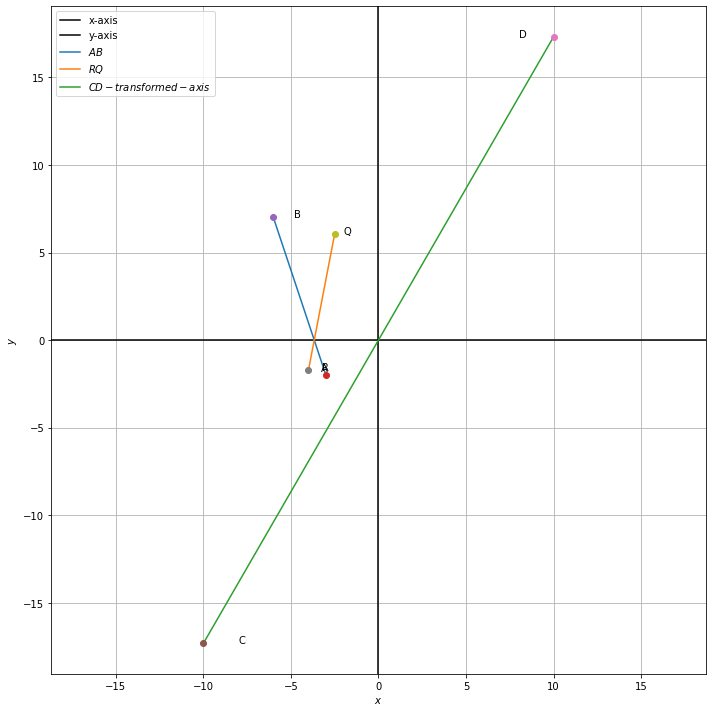
\includegraphics[width=\columnwidth]{image.png}
\caption{}
\label{fig:straight lines}	
\end{figure}
Distance between two points is 7.9372 
\end{document}
